\chapter{System Design}\label{system-design}

The design of Intelli-Trading Fours is driven by the central research
problem identified in Chapter 1: how to construct a system capable of
real-time, musically meaningful interaction with a human performer.
Chapter 2 discussed the existing approaches and limitations in both
offline generative systems and reactive accompaniment models,
particularly in their ability to sustain structured, interpretable
musical exchange. This section therefore establishes the design
principles that govern the system.

\section{Design Principles and System Framing}\label{design-principles-and-system-framing}

The design of Intelli-Trading Fours is driven by the requirement to
support real-time, musically meaningful interaction between a human
performer and an artificial agent. Rather than treating the system as a
standalone generator, it is framed as an interaction architecture in
which behaviour is defined by responsiveness to performer input.

Three principles govern this design:

\begin{enumerate}
\def\labelenumi{\arabic{enumi}.}
\item
  real-time operation constrains all decision-making to bounded temporal
  windows, favouring incremental and computationally lightweight
  processes over long-horizon optimisation.
\item
  interaction is structured rather than continuous, enabling clear
  segmentation of input and response and reducing ambiguity in timing
  and responsibility.
\item
  the system prioritises interpretability, exposing intermediate
  representations that make its behaviour understandable and
  controllable.
\end{enumerate}

These principles position the system as reactive rather than generative.
Outputs are not produced in isolation, but are shaped by the structure
of the performer's input within each interaction cycle. To support this,
the system adopts a symbolic representation of rhythm, enabling
tractable reasoning over temporal structure while maintaining alignment
with perceptual models of rhythmic organisation.

This framing establishes a controlled but flexible basis for human-AI
musical dialogue. It prioritises responsiveness, clarity and
evaluability, while accepting trade-offs in expressive nuance,
continuous interaction and stochastic variability.

\subsection{Interaction Model and Temporal Structure}\label{interaction-model-and-temporal-structure}

\begin{figure}[htbp]
\centering
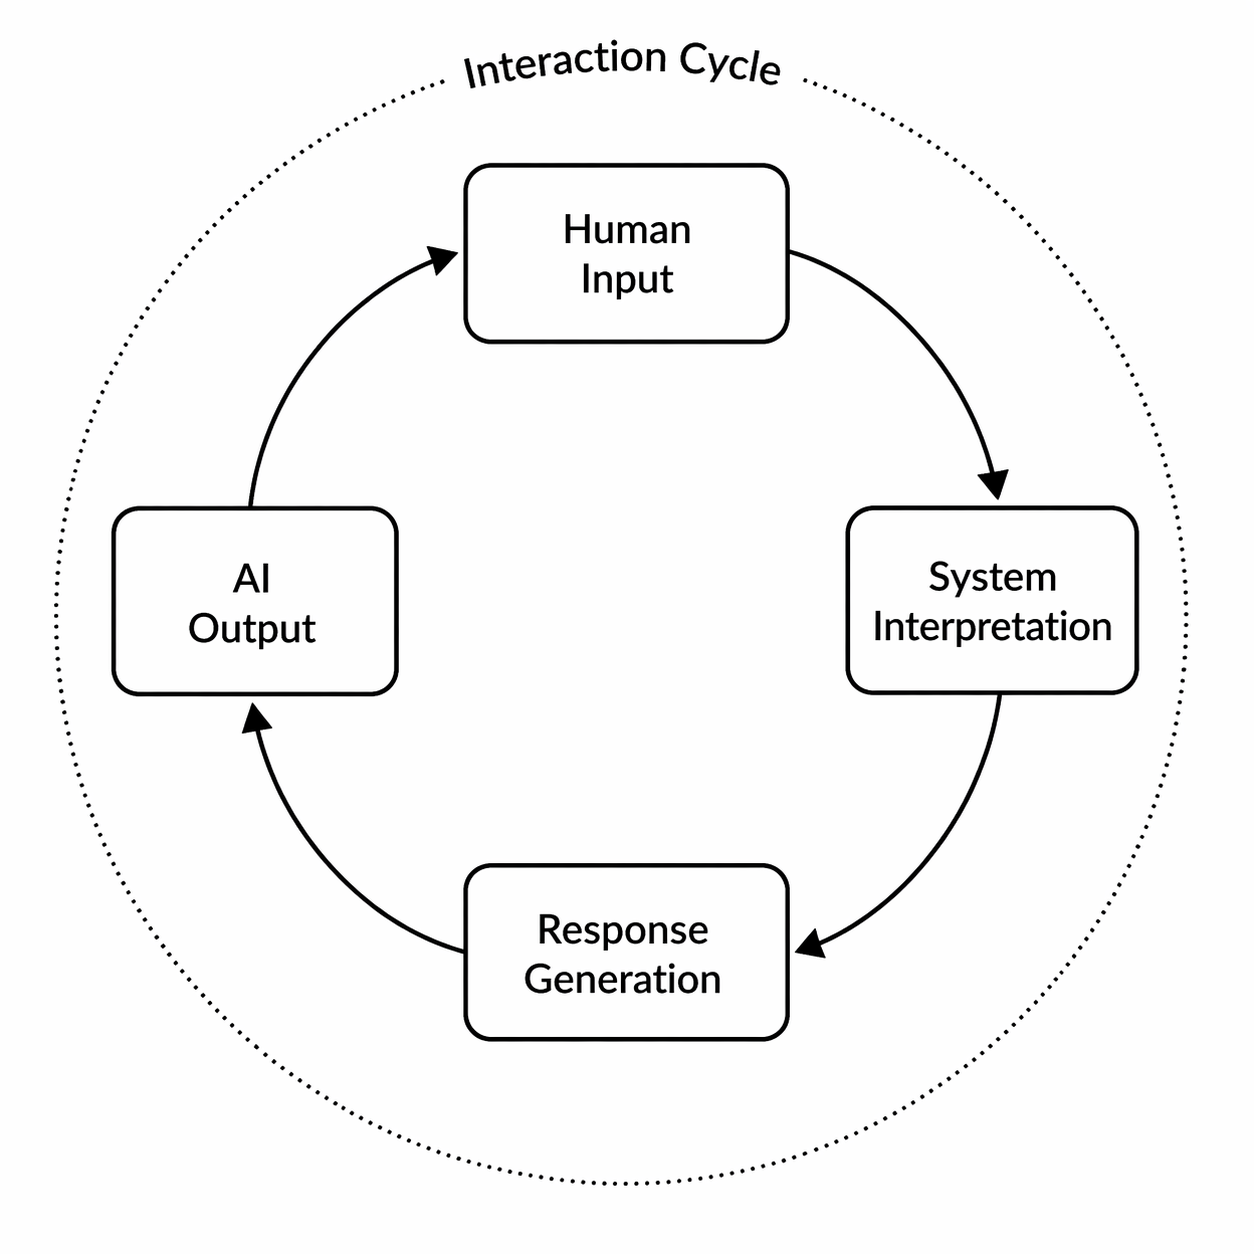
\includegraphics[width=\textwidth]{Figures/3 Figs/Closed-Loop Interaction Model.png}
\caption{Closed-loop interaction model illustrating the turn-based exchange between performer input and system response.}
\label{fig:closed-loop-interaction-model}
\end{figure}

The system is structured as a turn-based interaction loop in which human
input and system response occur in alternating cycles. This resolves the
temporal ambiguity of continuous co-improvisation by introducing
explicit boundaries for when input is interpreted and when responses are
produced.

Each cycle forms a bounded interaction unit. Input is treated as a
complete segment, allowing analysis and response to be performed within
a finite time window. This constraint supports real-time operation by
limiting the scope of computation and avoiding dependence on extended
performance history.

The model emphasises responsiveness over continuity. By enforcing
alternation, the system establishes a clear mapping between input and
response, improving interpretability and enabling direct evaluation of
system behaviour.

This design prioritises structural clarity and control, at the cost of
reduced expressive fluidity compared to continuous ensemble interaction.

\subsection{Symbolic Representation Strategy}\label{symbolic-representation-strategy}

\begin{figure}[htbp]
\centering
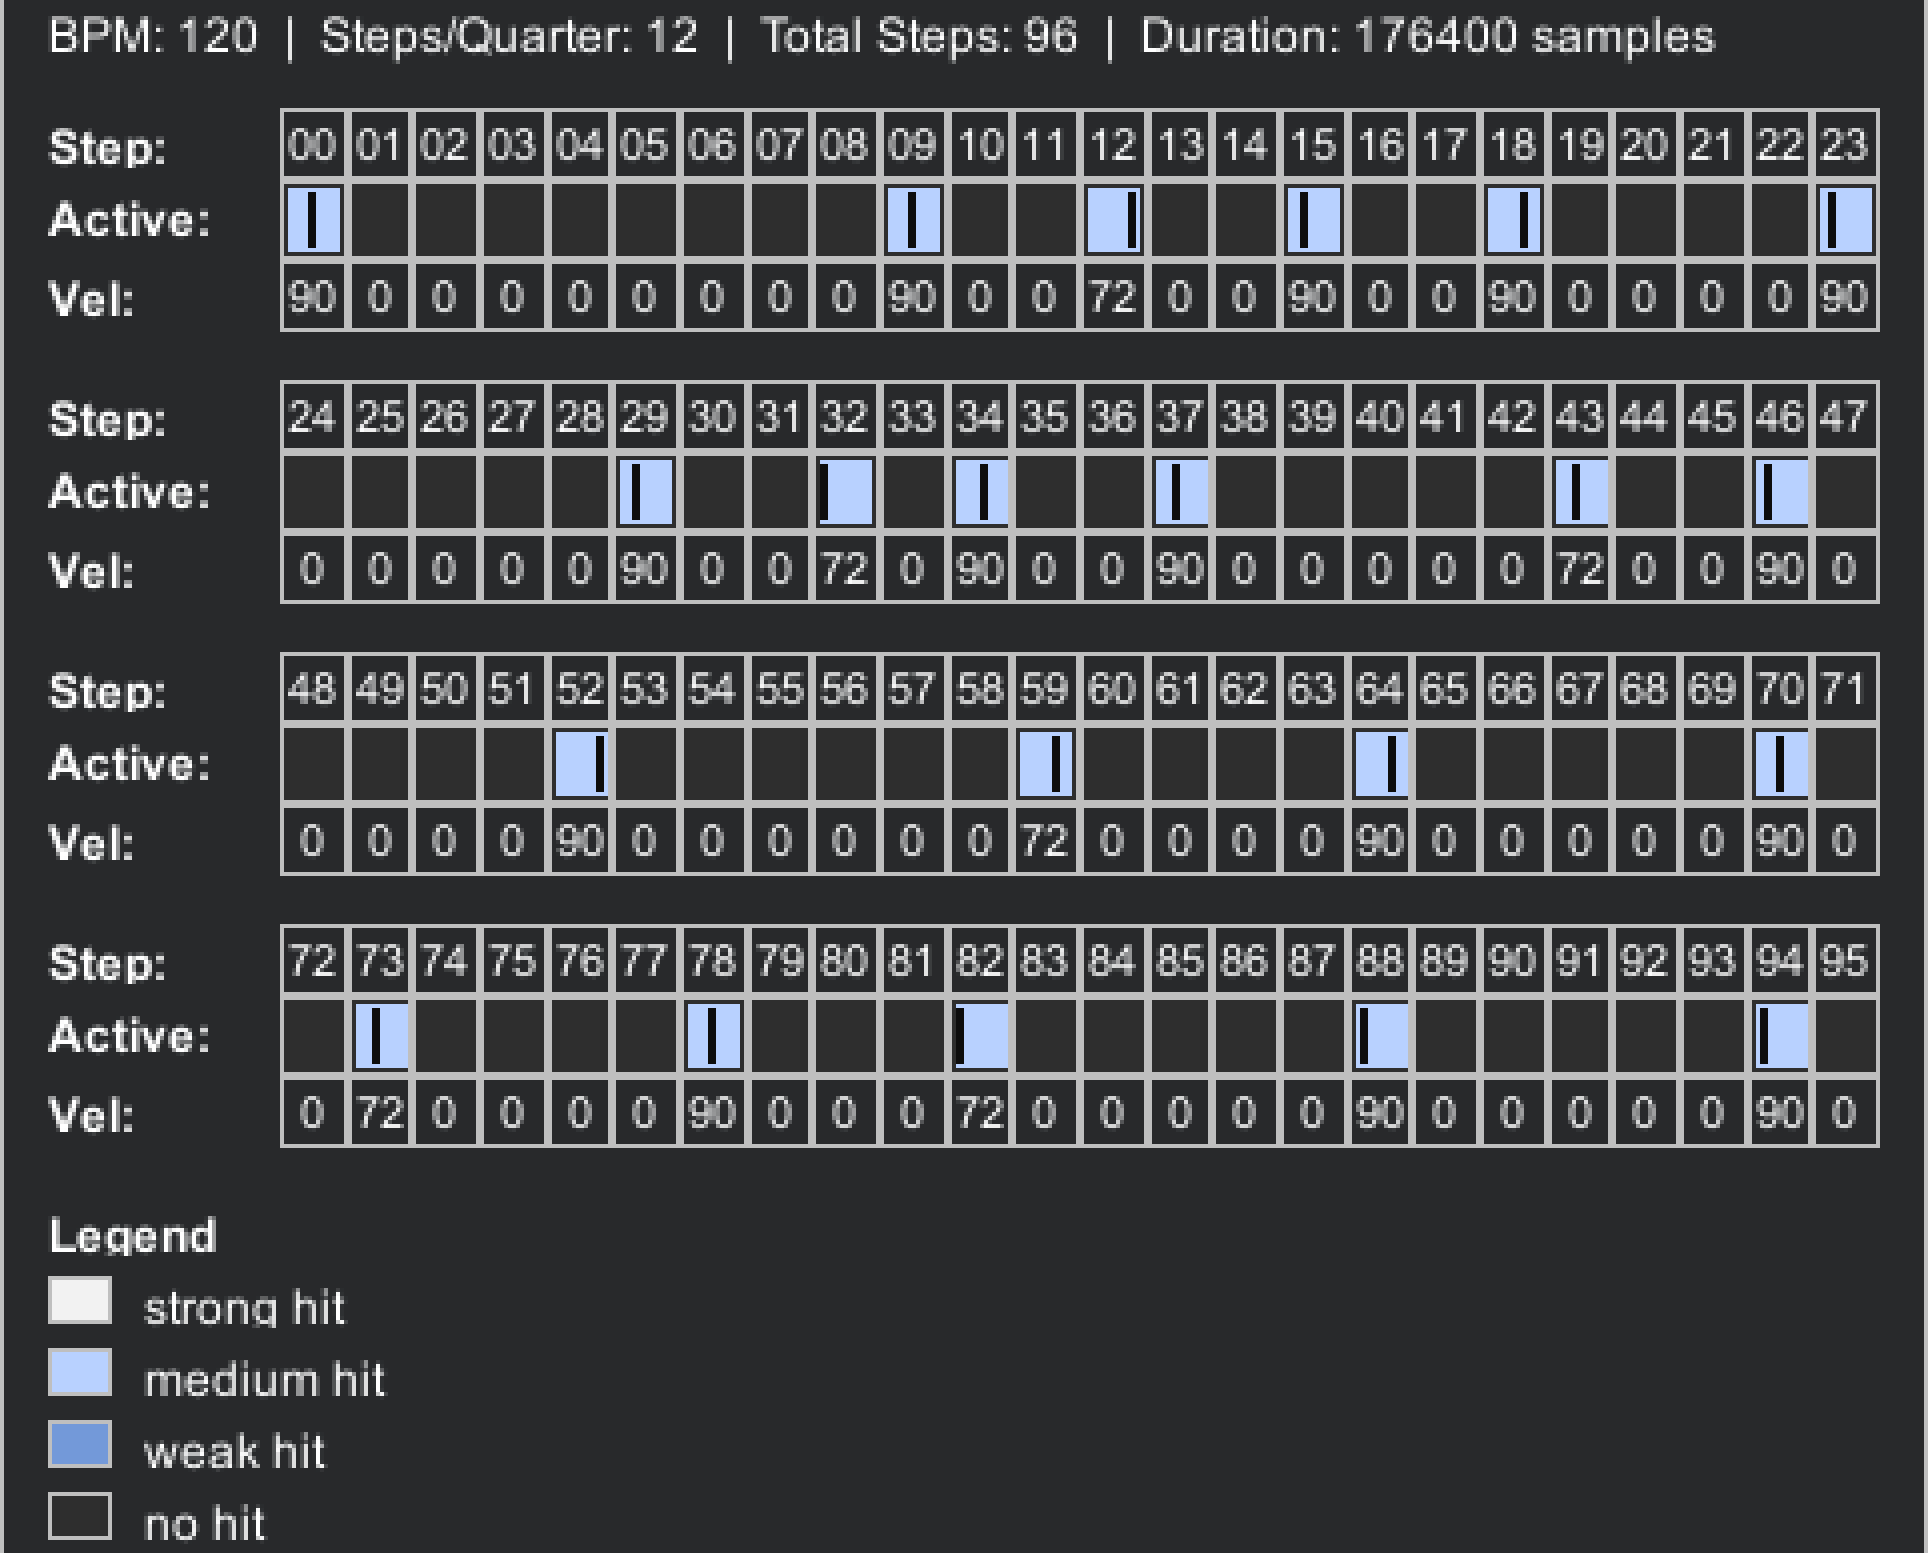
\includegraphics[width=\textwidth]{Figures/3 Figs/Symbolic Representation Strategy.png}
\caption{Symbolic representation strategy for converting performance input into a structured rhythmic form.}
\label{fig:symbolic-representation-strategy}
\end{figure}

The system represents performance using a symbolic, time-structured
abstraction rather than raw audio. Continuous input is mapped onto a
discrete temporal grid, allowing rhythmic events to be interpreted in
terms of relative timing, intensity and position within a structured
cycle.

This abstraction enables the system to reason about musical structure.
By imposing a consistent temporal framework, ambiguity in timing is
reduced and patterns such as density, emphasis and phrasing become
computationally accessible. This aligns with perceptual accounts of
rhythm, where listeners organise events according to metrical and
grouping structures.

The choice of symbolic representation prioritises tractability and
interpretability. It allows downstream processes to operate
deterministically on structured data, rather than relying on complex
signal-level analysis.

This design trades expressive nuance for clarity. Fine-grained timing
variation and timbral detail are simplified, but the resulting
representation supports consistent analysis and controllable response
generation.

\subsection{Interpretable Analysis and Planning}\label{interpretable-analysis-and-planning}

\begin{figure}[htbp]
\centering
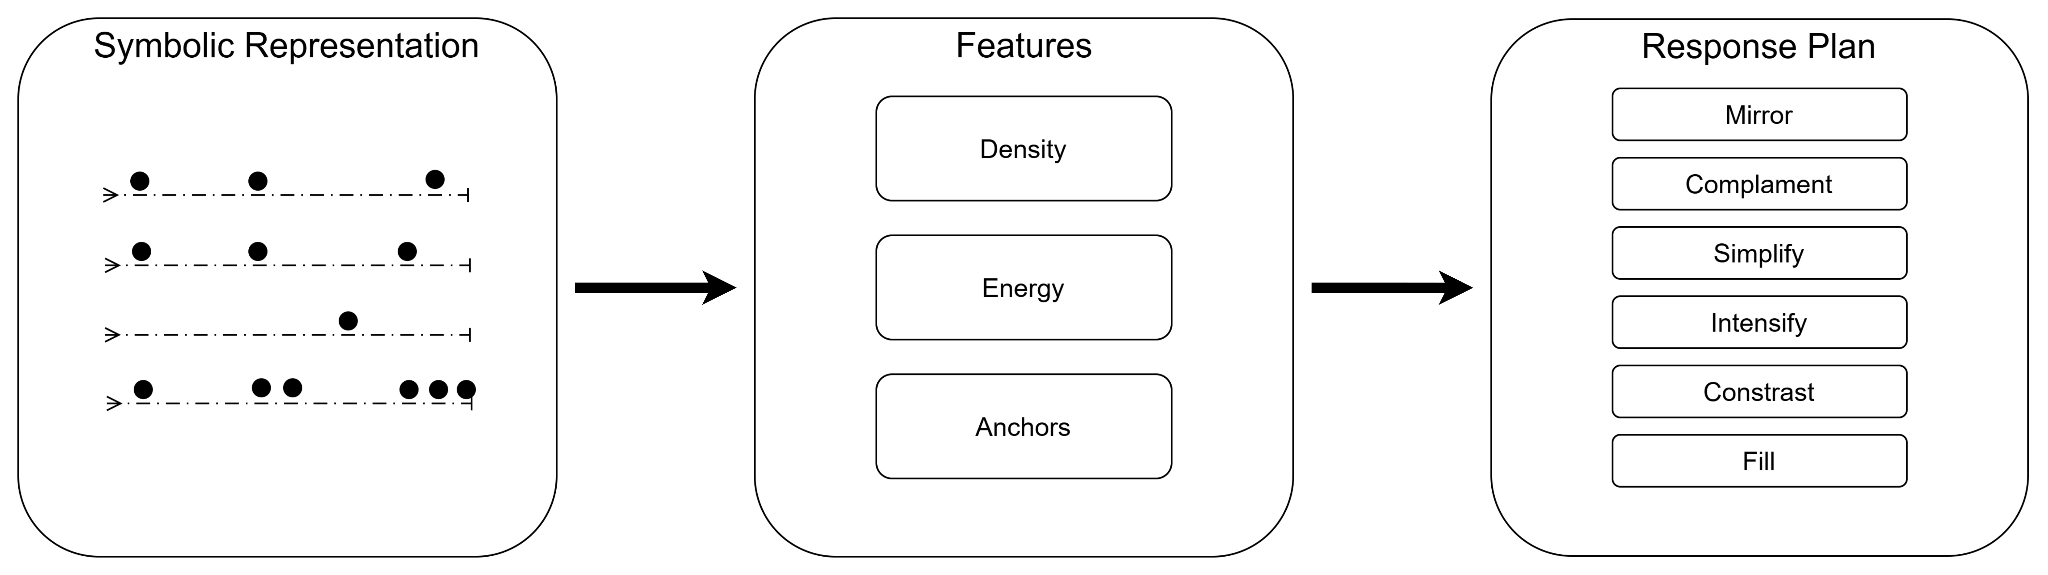
\includegraphics[width=\textwidth]{Figures/3 Figs/Analysis and Planning Pipeline.png}
\caption{Interpretable analysis and planning pathway from rhythmic input to response intent.}
\label{fig:analysis-planning-pipeline}
\end{figure}

The system derives meaning from input through a structured analysis and
planning process. Rather than directly transforming input into output,
it first extracts a set of interpretable descriptors capturing aspects
of rhythmic structure, such as activity, emphasis and distribution over
time.

These descriptors form the basis of a decision layer that determines how
the system should respond. Instead of producing output through opaque or
end-to-end methods, the system explicitly maps analysed input
characteristics to a small set of response behaviours, defining the
intended relationship between input and output.

This separation between analysis and planning supports interpretability.
Because decisions are expressed in terms of observable features and
discrete response types, system behaviour can be inspected, understood
and evaluated. This is particularly important in interactive settings,
where responsiveness must be both perceptible and explainable.

The design prioritises transparency and control over expressive
complexity. While this limits the richness of possible responses
compared to more implicit models, it ensures that responses remain
meaningfully grounded in the structure of the performer's input.

\subsection{Structural Response Generation and Output Coupling}\label{structural-response-generation-and-output-coupling}

\begin{figure}[htbp]
\centering
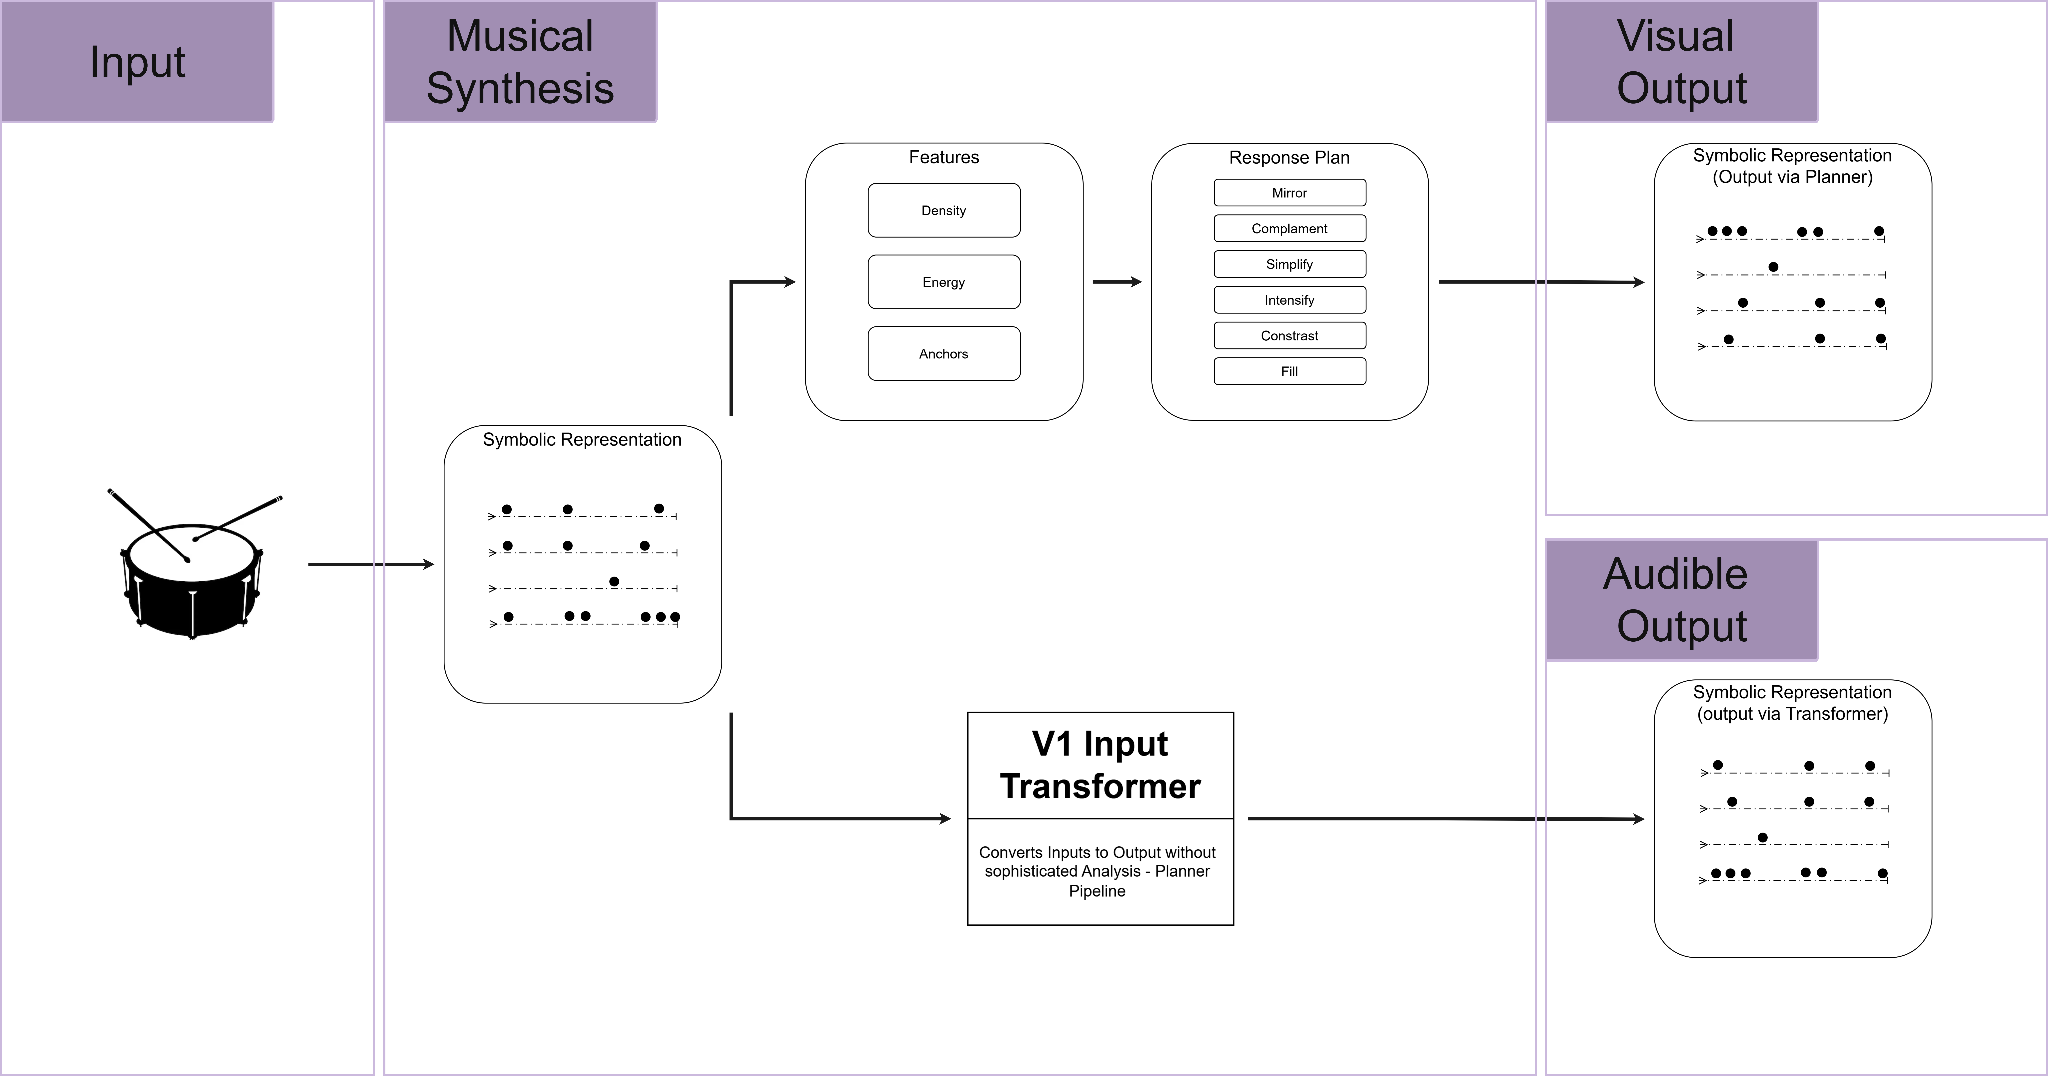
\includegraphics[width=\textwidth]{Figures/3 Figs/Structural Response Generation and Output Coupling.png}
\caption{Structural response-generation pathway and its current coupling to the audible output layer.}
\label{fig:structural-response-output-coupling}
\end{figure}

The system models response generation as a two-stage process: first
determining how to respond and then determining how that response is
realised. This distinction allows interaction to be defined in terms of
interpretable musical intent, rather than direct transformation of input
patterns.

As shown in Figure~\ref{fig:structural-response-output-coupling}, the intended design follows a reasoning pathway
from input analysis to response planning and from planning to a
structured rhythmic pattern. Within this framework, the system selects a
response strategy (e.g. mirroring, contrasting, extending) based on
extracted features and expresses this intent structurally by shaping the
distribution of events across the rhythmic grid. This establishes a
clear separation between decision-making and pattern construction,
supporting transparency and controllability in the interaction process.

However, the current output pathway diverges from this intended design.
Audible responses are not generated from the structural pattern, but
instead through a transformation process applied directly to the input
representation. As illustrated in the diagram, this results in a partial
coupling between structural reasoning and realised output.

This boundary is a defining characteristic of the current system. While
the architecture successfully implements an interpretable reasoning
framework, the translation from planned structure to audible behaviour
is not yet fully integrated. Consequently, the system's internal
decision-making is more developed than its external musical realisation.

This design reflects a deliberate prioritisation of interpretability and
structural clarity over immediate expressive completeness.
